\documentclass[twocolumn]{article}

\usepackage{graphicx}
\usepackage[doi=false,url=false,isbn=false]{biblatex}
\usepackage{microtype}
\usepackage[top=1in, bottom=1in, left=0.8in, right=0.8in]{geometry}
\usepackage{titlesec}
\usepackage{color}

% \usepackage{fontspec}
% \setmainfont{Humor Sans}

\graphicspath{{./images/}}

\title{\bfseries\fontsize{22}{1}\selectfont Open Benchmarks for Energy Measurements on Embedded Platforms}
\author{James Pallister, Simon Hollis, Jeremy Bennett}

\bibliography{refs}
\titleformat{\section}{\Large\bfseries\centering\scshape}{}{0em}{}
\titleformat{\subsection}{\normalsize\bfseries}{}{0em}{}

\newcommand{\nsection}[1]{\section{\bfseries #1}}
\newcommand{\todo}[1]{\textbf{\textcolor{red}{#1}}}

\begin{document}
\maketitle
\nsection{Abstract}

\textbf{This paper presents and justifies a benchmark suite targeted at embedded processors for evaluating energy consumption. The possible sources of energy consumption are considered and individual benchmarks selected from contemporary suites to cover key points affecting the energy consumption. The benchmark suite is portable, with six platforms considered. A subset of the platforms and benchmarks are extensively evaluated with instruction traces gathered and their instruction distributions analysed.}

\nsection{Introduction}

Benchmarking is frequently used to gain an idea of how a system will perform during its general use, when the specific environment cannot be reproduced at design-time. This gives designers feedback on how their system will perform and where its performance is lacking. Typically one benchmark cannot exercise all aspects of a target, leading to suites of benchmarks. Each benchmark tests a combination of areas of the hardware. This separation of benchmarks allows the design to see which parts of the hardware perform the best.

The energy consumption of our electronic devices is rapidly becoming a large factor in the design process. A portable embedded system will typically have severe power constraints placed upon it, if it is to have a long battery life. To recognise whether these constraints have been met, the power consumption of the device under a typical load must be tested. To build a full picture of a platform’s energy consumption characteristics, a benchmark suite that hits possible combinations of an applications characteristics (such as memory accesses, integer and floating point operations, etc) is needed. This allows the energy consumption of various components of the system to be determined, ensuring that the system is fit for purpose.

\begin{table*}[th!]
\centering
	\begin{tabular}{l c c c c c c c l}
	Name				 	& Source 	& B & M & I & FP& T 		& License & Category \\
	\hline
	Arithmetic Compression	& Other		& M & M & L & M & Single 	& GPL	& consumer, telecomm	\\
	FFT						& MiBench 	& M & H & L & H & Multi?	&  GPL	& automotive, telecomm	\\
	Patricia				& MiBench 	& H & H & L & L & Multi 	& GPL	& network	\\
	Primes					& WCET 		& M & L & H & L & Multi 	& None	& automotive	\\
	Triple-DES				& Other	 	& L & M & H & L & Multi 	& GPL	& security	\\
	\hline
	Blowfish				& MiBench 	& L & M & H & L & Multi 	& GPL	& security	\\
	CRC32					& MiBench 	& M & L & H & L & Single 	& GPL	& network, telecomm	\\
	Cubic root solver		& MiBench 	& L & M & H & L & Single 	& GPL	& automotive	\\
	Dijkstra				& MiBench 	& M & L & H & L & Multi 	& GPL	& network	\\
	FDCT					& WCET 		& H & H & L & H & Single 	& None	& consumer	\\
	Float Matmult			& WCET 		& M & H & M & M & Single 	& GPL	& automotive, consumer	\\
	Integer Matmult			& WCET	 	& M & M & H & L & Single 	& None	& automotive	\\
	Rjindael				& MiBench 	& H & L & M & L & Multi 	& GPL	& security	\\
	SHA						& MiBench 	& H & M & M & L & Multi 	& GPL	& network, security	\\
	2D FIR					& WCET 		& H & M & L & H & Single 	& None	& automotive, consumer	\\
	\end{tabular}
\caption{Benchmarks selected, and the categories they fit in. Benchmarks after the partition are examined in more detail. Legend in Table~\ref{BenchmarkLegend}.}
\label{Table:BenchmarkTable}
\end{table*}

Many benchmark suites exist already, such as MiBench\cite{Guthaus2001}, MediaBench\cite{Fritts2009}, LINPACK\cite{Dongarra2003}, Dhrystone\cite{Weicker1988} and more. These are all targeted towards larger desktop-based applications, with significant compute power. This is due to their emphasis on measuring performance, as opposed to energy efficiency. Most at least assume a host operating system, which may not be present on an embedded system. Further more, when analysing energy consumption, having to account for the operating system’s effect on the result is non-trivial. These benchmarks --- while in theory are portable --- have significant difficulties running unmodified on embedded platforms due to memory and storage constraints. The issue with portability also arises when it is necessary to constrast multiple platforms.

Currently a good benchmark suite for measuring energy consumption is not available for embedded platforms. MiBench is the closest in terms of variety of benchmarks and applicability but assumes there is a host operating system for the majority of the benchmarks. In particular it requires access to a filesystem which is usually unavailable on small embedded platforms.

In this paper a set of benchmarks chosen from popular benchmark suites is presented, along with justification for their use in benchmarking energy consumption. The benchmark suite is designed to expose the processor and memory's performance, with other factors such as IO and periphals excluded for portability. The selection was designed such that they benchmarks would be cross platform, exercising aspects of the processor and memory system. The benchmarks are intended to be run on the ‘bare metal’ with no host operating system.

We consider four orthogonal aspects that the benchmark suite must cover, allowing the range of benchmarks to expose all of the behavior of the platform.

\begin{itemize}
	\setlength{\itemsep}{-0.25em}
	% \vspace{-3mm}
	\item Floating point vs integer operations
	\item Memory access intensity
	\item Multithreaded-ness
	\item Branching frequency
\end{itemize}

Using benchmarks that hit combinations of these, interesting observations about the enery consumption of the device can be made.

Six different platforms are targetted by the benchmark suite. Targetting multiple platforms ensures that more general conclusions can be drawn about the nature of the energy consumption.
% \begin{itemize}
% 	\setlength{\itemsep}{-0.25em}
% 	% \vspace{-2mm}
% 	\item STM32F0DISCOVERY - ARM Cortex-M0
% 	\item STM32VLDISCOVERY - ARM Cortex-M3
% 	\item BeagleBone - ARM Cortex-A8
% 	\item Adapteva Epiphany
% 	\item XMOS L1
% 	\item ChipKIT Uno - PIC32MX (MIPS)
% \end{itemize}

\begin{center}
	\begin{tabular}{l l}
		Vendor  & Processor \\
		\hline
		ARM		& Cortex-M0 \\
		ARM		& Cortex-M3 \\
		ARM 	& Cortex-A8 \\
		Adapteva& Epiphany \\
		XMOS	& L1 \\
		Michrochip & PIC32MX (MIPS) \\
	\end{tabular}
\end{center}

\todo{concluding sentence.}

\nsection{Previous Work}

MiBench established a well known set of benchmarks with well characterised behaviour. This suite consisted of 37 different benchmarks split across six different categories, chosen to be representative of which applications would be run on both desktop and embedded platforms. Each benchmark is justified, with instruction traces analysed on a model of the StrongARM architecture. This gave a good overview of the proportions of each type of instructions that the benchmarks executed. The drawback of this was that the instruction traces were only gathered for one platform - each benchmark could have a radically different instruction distribution for alternative platforms.

MiBench was used as the main benchmark suite for MILEPOST GCC\cite{Fursin2011}. This study applied machine learning to predict which optimizations would benefit a program without needing to perform expensive iterative compilation techniques. In this study they emphasised how the performance acheived can be very dependent on the structure of the benchmarks. This highlights the need to have a wide range of benchmarks which each hit different combinations of the types of computation they could perform.

\begin{table}[t]
\centering
	\begin{tabular}{c l}
		Key & Description \\
		\hline
		L	&	Low \\
		M	&	Medium \\
		H	&	High \\
		\hline
		B	&	Branching \\
		M	&	Memory intensity \\
		I	&	Integer pipeline intensity \\
		FP	&	FPU pipeline intensity \\
		T	&	Threaded-ness \\
	\end{tabular}
	\caption{Legend for the benchmark table}
	\label{BenchmarkLegend}
\end{table}


\begin{table*}[!hbt]
	\centering
	\begin{tabular}{l l l l l}
		\textbf{Board name} & \textbf{Processor} & \textbf{RAM} & \textbf{Speed} & \textbf{Extra} \\
		\hline
		STM32F0DISCOVERY	& ARM Cortex-M0 		& 8KB		& 48 MHz		  & 64KB Flash\\
		STM32VLDISCOVERY	& ARM Cortex-M3 		& 8KB		& 24 MHz		  & 128KB Flash\\
		BeagleBone			& ARM Cortex-A8 		& 256MB		& 500 MHz		  & VFP/NEON, superscalar\\
		EMEK3				& Adapteva E16 			& 32KB/core & 400 MHz		  & FPU, superscalar, 16 core NoC\\
		XK1					& XMOS L1 				& 64KB		& 100 MHz 		& 4$\times$100MHz hardware threads \\
	\end{tabular}
	\caption{The platforms explored in this paper along with some relevant details.}
	\label{Table:Platforms}
\end{table*}
ParMiBench, a variant of MiBench was created to address the lack of multithreadedness in the original suite. This attempts to parallelise some of the benchmarks, allowing them to be used to benchmark multicore systems. This has an advantage over other parallel benchmark suites in that it also targets the embedded space. Very few other benchmark suites (such as LINPACK, PARSEC and SPLASH-2\cite{Bienia2008}) target multithreadedness at this level --- most are aimed at large clusters and HPC applications.

DSPstone\cite{Zivojnovic} is a benchmark suite for Digital Signal Processors (DSPs) and was originally designed to evaluated compiler effectiveness at compiling for DSPs. This suite contains a large amount of non-integer tests, with most tests replicated in fixed point and floating point form. As this set is aimed at DSPs rather than general purpose processors no benchmarks were chosen from DSPstone. The lack of an explicit license attached to these applications also makes it difficult to redistribute them under a single license.

A set of benchmarks is maintained by the worst case execution time (WCET) initiative\cite{Gustafsson2010}. These benchmarks are good because they are self contained and written completely in C. Each benchmark is less comprehensive than from the MiBench set, but focusses on one particular application that may be specifically what a low end processor will perform. Some of these applications fit well with typical embedded applications,

In addition to the previous benchmark suites, several other suites were evaluated. These were:
\begin{itemize}
	\setlength{\itemsep}{-0.25em}
	\item MediaBench
	\item OpenBench\cite{OpenBench}
	\item SPEC2006\cite{Henning2006}
	\item LINPACK
	\item Livermore Fortran Kernels
\end{itemize}

All of these benchmark suites were found to be unsuitable for the aim of characterising energy consumption on embedded platforms due to their reliance on the operating system and features provided by it.

\nsection{Platforms}

A range of platforms has been chosen, covering different types of architectures for different purposes. The processors are mainly small architectures which are designed for low power usage. As a consequence some of the platforms are very memory limited, restricting the types of applications that would be run on them.

A set of platforms is needed to complement the benchmark suite due to the varying capabilities of each platform. For example, a benchmark will behave very differently on platforms which have a cache, compared to platforms which do not. As such, we identified a number of parameters that should be varied to ensure the characterisation of the energy consumption is correct:

\begin{itemize}
	\setlength{\itemsep}{-0.25em}
	\item Caching
	\item Multi vs single core.
	\item Pipeline depth.
	\item Presence of an FPU.
	\item On chip vs off chip memory.
\end{itemize}

Table~\ref{Table:Platforms} summarises the platforms selected to represent combinations of the above parameters.

\nsection{Benchmarks}

A set of benchmark to to tests all aspects of the target platforms is presented in this section. The benchmarks were selected by defining a coverage matrix which included all the benchmarks from following suites:
\begin{itemize}
	\setlength{\itemsep}{-0.35em}
	\item MiBench
	\item DSPstone
	\item WCET
	\item Livermore Fortan Kernels
	\item Dhrystone/Whetstone
	\item MediaBench
\end{itemize}

This matrix evaluates each benchmark for various qualities, such as expected instruction distribtion, types of operations performed, licensing, program length and portability. The final set of benchmarks was chosen from this list to be a minimal set covering the range of different instruction distributions. This set is shown in Table~\ref{Table:BenchmarkTable}, along with the amount of each instruction category considered.

Individual tests from several different benchmark suites were considered. In particular MiBench has 37 well defined benchmarks, however a large proportion of these are targeted at much higher end platforms than chosen. This lead to a small subset of the MiBench benchmarks being selected. Several benchmarks were sourced from the WCET set. These tested small applications which could conceivably be ran by the platforms discussed earlier.

All but two benchmarks come from these two suites. The remaining two were found from other GPL-licensed applications to fill gaps in the suite. Arithmetic compression was chosen because compression algorithms are often included in benchmark suites (as it is a common operation that a system will perform) and it is an unusal type of compression. Triple-DES was chosen as another encryption algorithm to complement Rijndael and Blowfish.

MiBench divides the embedded processor applications into six categories: automotive, network, consumer, security, telecomms and office. The benchmarks selected broadly fit into these categories, however consumer and office in particular require the higher end embedded processors. This is due to the benchmarks running `off the shelf' programs such as ghostscript and rsynth.

The other applications considered were all found to be too time consuming to port to a small embedded system, or unnecessary for inclusion because other benchmarks performed a similar set of operations.


\nsection{Benchmark Descriptions}

This section talks about each benchmark, giving a short description of the benchmark and why it is included. A breakdown of the types of instructions in the benchmark is given for each platform.

\subsection*{Categories}

The benchmarks are divided into several categories, broadly covering the areas where these benchmarks may be used, or which area they best represent. These categories are the same as used in the MiBench paper. However some of the benchmarks are broad enough that the fit into several categories. A more accurate classification of the groups the benchmarks fit into is shown in the table of benchmarks (Table~\ref{Table:BenchmarkTable}).

\begin{center}
	\begin{tabular}{l p{0.55\linewidth}}
		Category &	Description \\
		\hline
		automotive 	& This category demonstrates the mathematical ability of the processor. \\
		consumer	& Embedded processors are frequently used in consumer applications, performing tasks such as audio and video decoding. \\
		network		& Processors in routers frequently perform the operations in this category. This involves handling packets and routing graphs. \\
		telecomm	& Applications that include radio frequency analysis and encoding. \\
		security	& Encryption algorithms, hashing and signing applications are placed in this category. \\
	\end{tabular}
\end{center}

\vspace{3mm}
\textbf{Blowfish}\\
Blowfish is an encryption algorithm commonly used in cryptography. This benchmark was taken from MiBench but modified to encrypt small blocks of data, as if the data was being streamed into the processor. Encryption typically involves many integer operations with fewer, predictable branches.

\vspace{3mm}
\textbf{Rijndael}\\
Rijndael is the algorithm for the Advanced Encryption Standard. It is commonly used in many security applications, and has a similar structure to blowfish.

\vspace{3mm}
\textbf{Triple-DES}\\
TripleDES is an older encryption algorithm, similar to blowfish and Rijndael.

\vspace{3mm}
\textbf{SHA}\\
Secure Hashing Algorithm (SHA) is a hashing algorithm commonly used for fingerprinting and verification of data streams. It is useful for stressing integer pipelines, and has low memory requirements.

\vspace{3mm}
\textbf{CRC32}\\
Similar to SHA, CRC32 is used for verification of data streams, notably ethernet frames. It differs from SHA in that it can be implemented with very few instructions as it consists mainly of shifts and XORs.

\vspace{3mm}
\textbf{Primes}\\
The primes benchmark implements a prime seive. This benchmark is a more contrived example than others, which would be found in real applications more often. However, it is structured differently to the other integer benchmarks, so provides a useful comparison.

\vspace{3mm}
\textbf{Integer Matmult}\\
Integer matrix multiplication is used very frequently in many applications, and so is a useful benchmark to have. It consists of a tight inner loop with many array accesses, making it useful for stressing the memory and integer pipeline at the same time. This should also expose data caching effects of the platform.

\vspace{3mm}
\textbf{Float Matmult}\\
Floating point matrix multiplication is also used frequently. This benchmark is exactly the same as the integer matrix multiplication, but with floating point numbers. This should allow a good metric of relative performance between the integer and floating point pipeline to be produced.

\vspace{3mm}
\textbf{Arithmetic Compression}\\
Arithmetic compression is an entropy encoding that can be used to compress data.

\vspace{3mm}
\textbf{Dijkstra}\\
This benchmark implements the dijkstra shortest-algorithm path. This benchmark performs lots of non-linear accesses to memory, and branches unpredictably. This makes it good for stressing caches and branch units that the processor may have. This algorithm is commonly used by routers to calculate the shortest path to another router.

\vspace{3mm}
\textbf{Patricia}\\
This benchmark is similar to dijkstra in structure. It is also used in routers to compress sparse trees. Patricia performs less computation, but stores more complicated data structures in memory, possibly exercising the data caching abilities.

\vspace{3mm}
\textbf{Cubic root solver}\\
This benchmark performs a large amount of trigonometry to solve various cubic equations. This tests the floating point pipeline with very little memory required.

\vspace{3mm}
\textbf{2D FIR}\\
FIR filters are frequently using in image transformations. In the embedded space this could be the type of operations done by digital cameras. This benchmark is similar to the matrix multiplications but with potentially more memory accesses.

\vspace{3mm}
\textbf{FFT}\\
The FFT is used in many applications requiring frequency analysis of data. This is a standard algorithm often used as a benchmark, which makes it useful to be included in this set. This benchmark should stress the caches, as well as the floating point pipeline due to the butterfly type memory accesses it performs.

\vspace{3mm}
\textbf{FDCT}\\
This benchmark was included as it is a core algorithm behind many video decoders used in consumer products. This benchmark represents real-world usage of the systems as well as testing the floating point pipeline and caches.

\begin{figure}[t]
	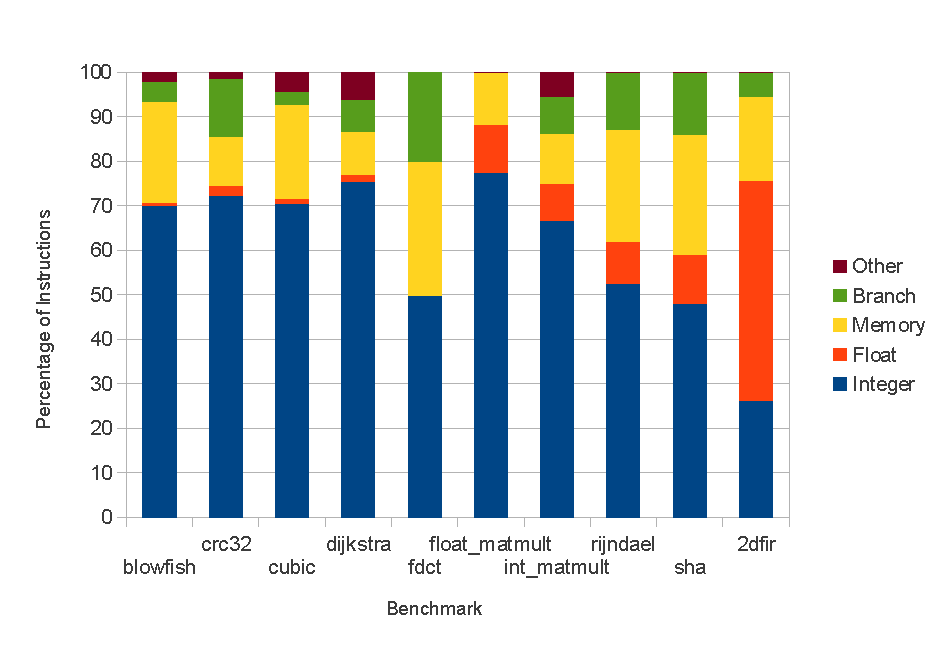
\includegraphics[width=\linewidth]{epiphany.pdf}
	\caption{Instruction distribution for the Epiphany platform.}
	\label{Fig:InstructionDistributionEpiphany}
\end{figure}

\begin{figure}[t]
	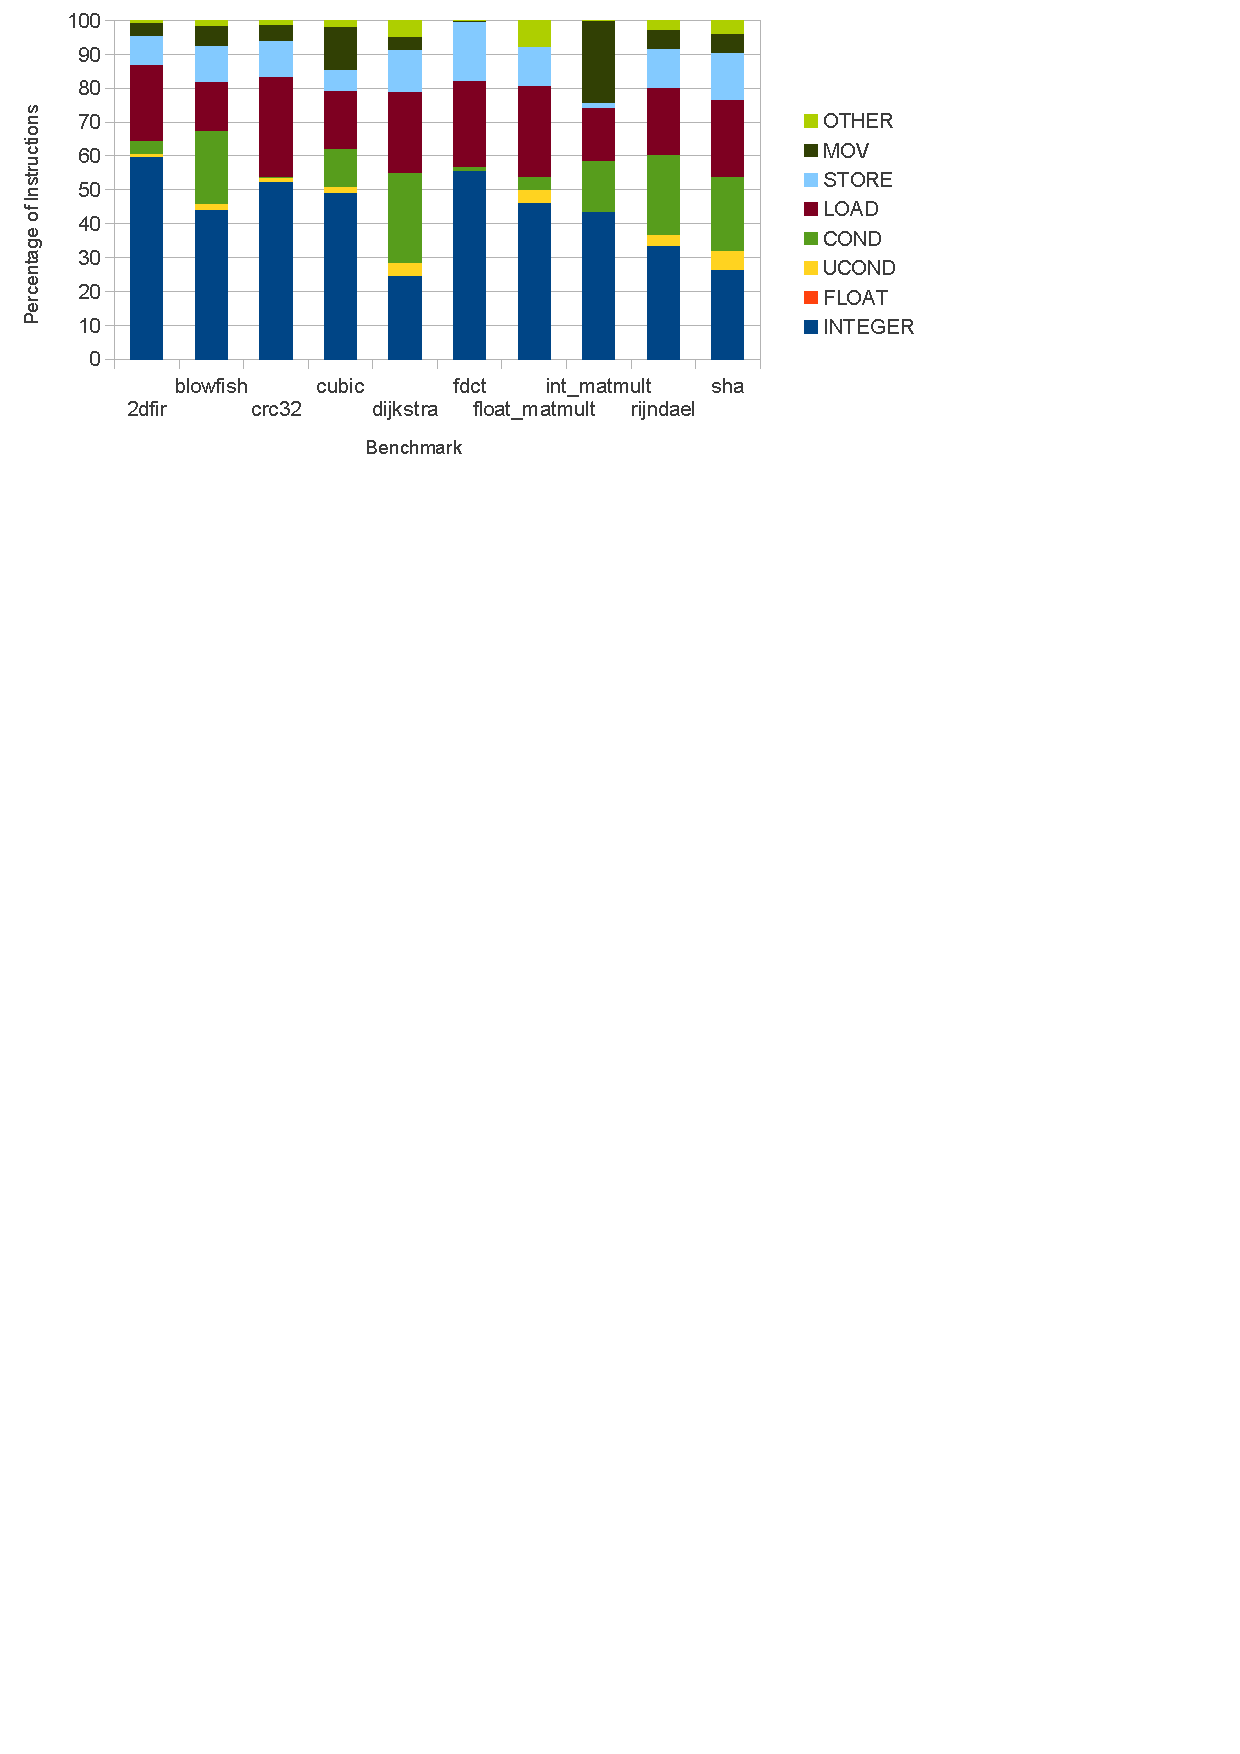
\includegraphics[width=\linewidth]{xmos.pdf}
	\caption{Instruction distribution for the XMOS platform.}
	\label{Fig:InstructionDistributionXMOS}
\end{figure}

\begin{figure}[t]
	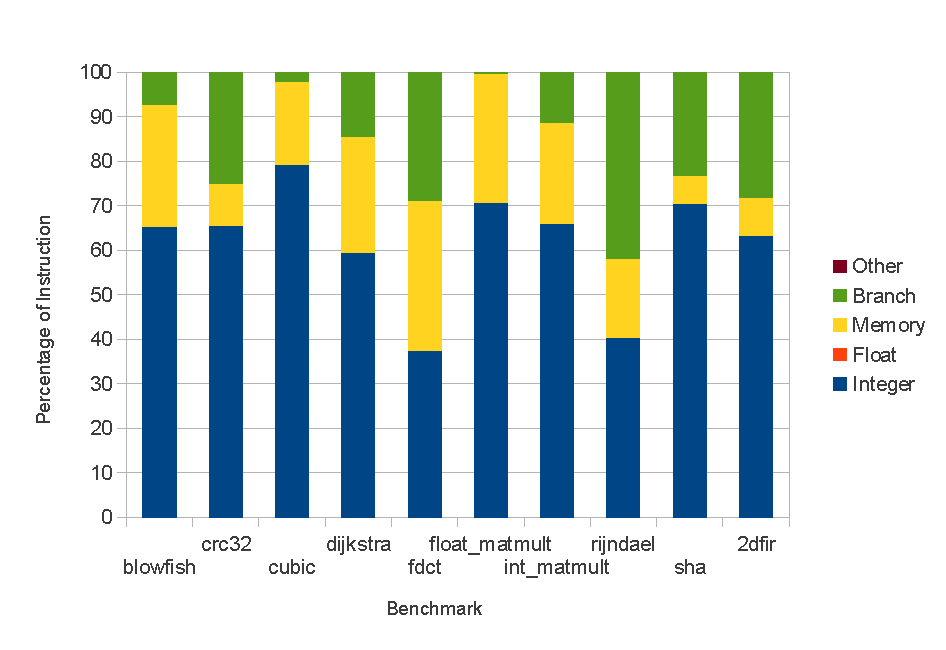
\includegraphics[width=\linewidth]{arm.pdf}
	\caption{Instruction distribution for the ARM Cortex-M0 platform.}
	\label{Fig:InstructionDistributionARM}
\end{figure}
sudo

\nsection{Benchmark Analysis}

A subset of the benchmarks were analysed by collecting their instruction traces across three of the platforms. From these graphs the instructions could be categories to ensure that each benchmark performed a different distribution of operations. Figures~\ref{Fig:InstructionDistributionEpiphany}, \ref{Fig:InstructionDistributionXMOS} and \ref{Fig:InstructionDistributionARM} show the instruction distributions for the Epiphany, XMOS and ARM Cortex-M0 (Thumb instruction set) platforms respectively. The `Other' category of instructions contains miscellaneous control instructions that do not fit into other categories (for example, interrupt control on the Epiphany platform).

Integer operations are the most common type of instruction in almost every benchmark. Across the platforms, the distributions are similar, with small variations due to the underlying instruction set. For example, there are a larger percentage of \texttt{mov}-type instructions in the Epiphany results because there are several predicated \texttt{mov} instructions (\texttt{moveq}, \texttt{movlt}, etc). This reduces the need for conditional branches, so this category decreases in proportion.

The ARM traces follow the same general trend as the traces for XMOS and Epiphany, however with overall less memory operations. This is due to the ARM processor having support for the \texttt{ldm} and \texttt{stm} instruction allowing multiple accesses to memory in a single instruction.
\todo{Some more discussion about the traces}

The integer instruction category is the largest group in almost every case, for all platforms and benchmarks. This category, however, includes the most different types of instructions, as it groups arithmetic, register copying and bit-wise operations. The individual instructions in each category is listed below.

\todo{is this useful? perhaps not.}

\begin{center}
	\begin{tabular}{l l l l}
		Category 	& Epiphany  & XMOS 	& ARM \\
		\hline
		Integer	 	& 27	  	& 23	& 22  \\
		Float		& 4			& 0		& 0	  \\
		Memory		& 8			& 7		& 11  \\
		Branch		& 23		& 7		& 16  \\
	\end{tabular}
\end{center}

\todo{Summarise the results. why do these results make it a good benchmark suite - varied distribution, similarities across platforms but differences to (as you would expect, with different hardware). Talk about how the hardware contributes to the difference in the results}

\nsection{Evaluation}

\todo{With base energy measurements for each instruction, estimate amount of energy each benchmark should take from proportion of instructions. Compare these to actual figures from the benchmarks being run?}

\nsection{Conclusion}

This paper has presented a benchmark suite that has been designed to expose the energy consumption characteristics of the target platform. We tested it on three separate platforms allowing the orthongality of the benchmark's profiles to be examined. The benchmarks were found to have widely varying behavior making them ideal for their purpose. \todo{}

\printbibliography

\end{document}
